\documentclass{article}

%====================================================
%                  PACKAGES
%====================================================
\usepackage{graphicx}
\usepackage{subcaption}
\usepackage{fancyhdr}
\usepackage[margin=1in]{geometry}
\usepackage{listings}
\usepackage[hidelinks]{hyperref}
\usepackage{amsmath,amssymb,mathtools}
\usepackage{float}
\usepackage{lmodern}
\usepackage{xcolor}
\usepackage{fvextra}
\usepackage{longtable}
\usepackage{enumitem}
\usepackage{booktabs}
\usepackage{array}
\usepackage{multirow}
\usepackage{colortbl}
\usepackage{titlesec}
\usepackage{tikz}
\usepackage{eso-pic} 
\usepackage[most]{tcolorbox}
\usepackage{xepersian}
\usetikzlibrary{calc} 

%====================================================
%                  COLORS
%====================================================

\definecolor{softgreen}{RGB}{240,250,245}
\definecolor{mygreen}{RGB}{46,139,87}

\definecolor{softorange}{RGB}{255,248,235}
\definecolor{golden}{RGB}{218,165,32} 

\definecolor{softpink}{RGB}{255,240,245}
\definecolor{softred}{RGB}{205,92,92}

\definecolor{softgray}{RGB}{248,248,248}
\definecolor{glassbg}{RGB}{255,255,255} 
\definecolor{mainblue}{RGB}{15,76,129}
\definecolor{lightblue}{RGB}{226,238,250}
\definecolor{deepblue}{RGB}{9,24,51} 

% --- رنگ‌های جدید تم کلاسیک و پلاتینی صفحه اول ---
\definecolor{midnight}{RGB}{8, 12, 20}         % سورمه‌ای/مشکی بسیار تاریک و عمیق
\definecolor{platinum}{RGB}{214, 219, 223}     % نقره‌ای روشن و شیک برای متن و لبه‌ها
\definecolor{mutedslate}{RGB}{69, 84, 104}     % خاکستری متمایل به آبی برای فریم‌ها و کادرها
\definecolor{slatebg}{RGB}{20, 30, 45}          % سورمه‌ای-زغالی عمیق و مات

\definecolor{softgray}{RGB}{245,245,245}

% تم کادرهای مات
\definecolor{mattedarkblue}{RGB}{35, 45, 60} 
\definecolor{mattebgblue}{RGB}{248, 250, 253} 
\definecolor{mattedarkgold}{RGB}{120, 95, 45} 
\definecolor{mattebggold}{RGB}{254, 253, 249} 
\definecolor{mattedarkred}{RGB}{100, 35, 40} 
\definecolor{mattebgred}{RGB}{253, 248, 248} 

% رنگ‌های تم VS Code Dark+
\definecolor{vscBackground}{RGB}{30,30,30}      
\definecolor{vscText}{RGB}{212,212,212}         
\definecolor{vscPink}{RGB}{197,134,192}         
\definecolor{vscBlue}{RGB}{86,156,214}          
\definecolor{vscString}{RGB}{206,145,120}       
\definecolor{vscComment}{RGB}{106,153,85}       
\definecolor{vscTopBar}{RGB}{37,37,38}          


%====================================================
%                  HYPERREF
%====================================================
\hypersetup{
	colorlinks=true,
	linkcolor=mainblue, 
	filecolor=magenta,
	urlcolor=mainblue, 
	citecolor=mygreen 
}

%====================================================
%                  FONTS
%====================================================
\settextfont[Path={./font/}, Scale=1.4]{IRLotus}
\setlatintextfont[Scale=1.1]{Times New Roman}

%====================================================
%                  PAGE STYLE
%====================================================
\setlength\headheight{28pt}
\pagestyle{fancy}
\fancyhf{}
\lhead{\textcolor{mainblue}{\textbf{پروژه هوش مصنوعی}}}
\chead{
\includegraphics[width=1cm,height=1cm,keepaspectratio]{img/Logo.png}}
\rhead{\textcolor{mainblue}{\textbf{\thepage}}}
\rfoot{\textcolor{gray}{حامد بهروزی مقدم - علیرضا دیوسالار}}
\renewcommand{\headrulewidth}{1.5pt} 
\renewcommand{\headrule}{\hbox to\headwidth{\color{mainblue}\leaders\hrule height \headrulewidth\hfill}}
\renewcommand{\footrulewidth}{1pt}
\renewcommand{\footrule}{\hbox to\headwidth{\color{gray}\leaders\hrule height \footrulewidth\hfill}}

%====================================================
%                  SECTION STYLE
%====================================================
\titleformat{\section}
{\Large\bfseries\color{mainblue}}
{\begin{tikzpicture}[baseline={(0,-0.1)}]
		\node[fill=mainblue,text=white,rounded corners=2pt,inner sep=4pt] {\thesection};
\end{tikzpicture}}
{0.5em}
{}[\vspace{0.2ex}\titlerule] 

\titlespacing{\section}{0pt}{20pt}{10pt} 

%====================================================
%                  LINE SPACING & LISTINGS
%====================================================
% ====================================================
%       4. VS CODE STYLE DEFINITION
% ====================================================

% --- استایل پایتون (همان استایل قبلی) ---
\lstdefinestyle{vscode_inner}{
    language=Python,
    backgroundcolor=\color{vscBackground},
    basicstyle=\linespread{1.1}\ttfamily\footnotesize\color{vscText}, 
    commentstyle=\color{vscComment}\itshape,
    stringstyle=\color{vscString},
    numberstyle=\tiny\color{gray}, 
    breakatwhitespace=false,
    breaklines=true,
    keepspaces=true,
    numbers=left,
    numbersep=12pt, 
    showspaces=false,
    showstringspaces=false,
    showtabs=false,
    tabsize=4,
    frame=none, 
    xleftmargin=12pt,
    morestring=[s]{"""}{"""},
    morestring=[s]{'''}{'''},
    classoffset=0,
    morekeywords={def,for,in,return,class,if,else,elif,while,try,except,with,and,or,not,is,yield,global},
    keywordstyle=\color{vscPink}\bfseries,
    classoffset=1,
    morekeywords={import,as,from,True,False,None,self,pass,print},
    keywordstyle=\color{vscBlue}\bfseries,
    classoffset=0, 
}

% --- محیط‌های نمایش کد (هر دو) ---
\newtcblisting{vscodewindow}[1]{
    enhanced,
    listing only,
    listing options={style=vscode_inner},
    title={\tikz[baseline=-0.6ex]{\fill[red!80!white] (0,0) circle (3.5pt); \fill[yellow!90!black] (0.4,0) circle (3.5pt); \fill[green!80!black] (0.8,0) circle (3.5pt);} \hspace{10pt} \ttfamily\footnotesize #1}, 
    fonttitle=\sffamily,
    coltitle=white,
    colbacktitle=vscTopBar, 
    colframe=vscTopBar, 
    colback=vscBackground,
    coltext=vscText, 
    arc=5mm, 
    outer arc=5mm,
    boxrule=1pt,
    titlerule=0pt, 
    toptitle=3mm, 
    bottomtitle=3mm,
    top=3mm, 
    bottom=3mm,
    left=2mm,
    right=2mm,
    drop shadow=black!50!white, 
    before skip=15pt,
    after skip=15pt
}
%====================================================
%                  TCOLORBOX
%====================================================
\tcbset{
	enhanced,
	breakable,
	arc=3mm, 
	boxrule=1pt, 
	fonttitle=\bfseries\large, 
	drop fuzzy shadow 
}

%====================================================
%                  AUTOREF
%====================================================
\AtBeginDocument{
	\def\chapterautorefname{فصل}%
	\def\sectionautorefname{بخش}%
	\def\subsectionautorefname{زیربخش}%
	\def\equationautorefname{رابطه}%
	\def\figureautorefname{شکل}%
	\def\tableautorefname{جدول}%
}

%====================================================
%                  DOCUMENT
%====================================================

\begin{document}
	
%====================================================
%                  TITLE PAGE (PROJECT 2)
%====================================================

    \begin{titlepage}
        \AddToShipoutPictureBG*{
            
\begin{tikzpicture}[remember picture,overlay]
                % پس‌زمینه دارک بسیار عمیق
                \shade[inner color=midnight!80!gray, outer color=midnight] 
                (current page.south west) rectangle (current page.north east);
                
                % گرید (چهارخانه) مهندسی بسیار محو در بک‌گراند
                \draw[mutedslate, opacity=0.08, step=0.8cm, thin] 
                (current page.south west) grid (current page.north east);
                
                % کادر دوبل نقره‌ای مات و کلاسیک
                \draw[mutedslate, line width=1.2pt, opacity=0.8] 
                ($(current page.north west)+(1.2cm,-1.2cm)$) rectangle ($(current page.south east)+(-1.2cm,1.2cm)$);
                \draw[platinum, line width=0.5pt, opacity=0.3] 
                ($(current page.north west)+(1.4cm,-1.4cm)$) rectangle ($(current page.south east)+(-1.4cm,1.4cm)$);
                
                % گوشه‌های مینیمال و شیک (استایل براکت)
                \draw[platinum, thick, opacity=0.8] ($(current page.north west)+(1.2cm,-2.5cm)$) -- ($(current page.north west)+(1.2cm,-1.2cm)$) -- ($(current page.north west)+(2.5cm,-1.2cm)$);
                \draw[platinum, thick, opacity=0.8] ($(current page.north east)+(-1.2cm,-2.5cm)$) -- ($(current page.north east)+(-1.2cm,-1.2cm)$) -- ($(current page.north east)+(-2.5cm,-1.2cm)$);
                \draw[platinum, thick, opacity=0.8] ($(current page.south west)+(1.2cm,2.5cm)$) -- ($(current page.south west)+(1.2cm,1.2cm)$) -- ($(current page.south west)+(2.5cm,1.2cm)$);
                \draw[platinum, thick, opacity=0.8] ($(current page.south east)+(-1.2cm,2.5cm)$) -- ($(current page.south east)+(-1.2cm,1.2cm)$) -- ($(current page.south east)+(-2.5cm,1.2cm)$);
            \end{tikzpicture}
        }
        
	
                      \begin{center}
                          \vspace*{1.2cm} 
                          
                          % عنوان اصلی با رنگ سفید درخشان
                          {\fontsize{42}{48}\selectfont \textbf{\textcolor{white}{گزارش پروژه دوم هوش مصنوعی}}} 
                          
                          \vspace{0.6cm} 
                          
                          % نام درس با رنگ پلاتینی
                          {\LARGE \textbf{\textcolor{platinum}{بازشناسی و طبقه‌بندی علائم ترافیکی آلمان (GTSRB)}}} 
                          
                          \vspace{0.4cm}
                          \textcolor{mutedslate}{\rule{5cm}{1pt}} % خط جداکننده نقره‌ای تیره
                          
                          \vspace{0.8cm} 
                         
                          % کادر لوگو - دارک و شیک (اصلاح شد)
                          \begin{tcolorbox}[
                              colback=black,         % اصلاح شد: همرنگ پس‌زمینه
                              colframe=black,        % اصلاح شد: همرنگ پس‌زمینه (حذف کادر)
                              boxrule=0pt,             % حذف کادر ضخیم
                              arc=4mm,             
                              left=3mm, right=3mm, top=3mm, bottom=3mm, 
                              width=0.22\textwidth, 
                              halign=center,
                              no shadow                % حذف سایه برای یکدست شدن
                              ]
                              
\includegraphics[width=\linewidth]{img/Logo.png}
                          \end{tcolorbox}
                          
                          \vspace{0.8cm} 
                          
                          % کادر عنوان فرعی با پلاک شناور مات
                          \begin{tcolorbox}[
                              width=0.85\textwidth,
                              colback=midnight!60!black, % پس‌زمینه شیشه‌ای و تاریک
                              colframe=mutedslate, 
                              arc=3mm, 
                              boxrule=1pt, 
                              title={\centering \Large \textbf{\textcolor{white}{فاز دوم پروژه پایانی}}}, 
                              fonttitle=\bfseries,
                              boxed title style={colback=mutedslate, colframe=mutedslate, arc=2mm}, % پلاک پلاتینی بالا
                              attach boxed title to top center={yshift=-12pt}, % شناور کردن پلاک
                              halign=center,
                              shadow={2mm}{-2mm}{0mm}{black!80} 
                              ]
                              \vspace{10pt}
                              \large
                              \textcolor{platinum}{طراحی، پیاده‌سازی و ارزیابی جامع شبکه عصبی پرسپترون چندلایه \lr{(MLP)} و شبکه عصبی پیچشی عمیق \lr{(CNN)} به همراه تحلیل ماتریس درهم‌ریختگی و آزمون مستقل بر روی داده‌های جدید.}
                            
                          \end{tcolorbox}
                          
                          \vspace{0.8cm} 
                          
                          % کادر اطلاعات دانشجو - دارک با نوشته‌های نقره‌ای و سفید
                          \begin{tcolorbox}[
                              width=0.75\textwidth,
                              colback=midnight!70!black, 
                              colframe=mutedslate, 
                              arc=3mm,
                              boxrule=1pt,
                              halign=center,
                              shadow={2mm}{-2mm}{0mm}{black!80} 
                              ]
                              \renewcommand{\arraystretch}{1.8} 
                              \large
                              \begin{tabular}{>{\bfseries\color{platinum}}c c} 
                               
                                                   نام دانشجو: & \textcolor{white}{حامد بهروزی مقدم - علی رضا دیوسالار} \\
                                                   شماره دانشجویی: & \textcolor{white}{40215633 - 40217493} \\
                                                   استاد درس: & \textcolor{white}{ جناب آقای دکتر علیاری} \\
                                             	لینک کد پروژه: & \href{https://colab.research.google.com/drive/1pwcG3xzuy7rzUewGk51ceqNiHa9ftft3#scrollTo=1aKB7h_dIRhi}{\lr{Google Colab}} \\
                                             				لینک دیتاست پروژه: & \href{https://www.kaggle.com/datasets/meowmeowmeowmeowmeow/gtsrb-german-traffic-sign}{\lr{Kaggle Dataset}} \\
                              \end{tabular}
                          \end{tcolorbox}
                          
                      \end{center}
\end{titlepage}
	
	%====================================================
	%                  TABLE OF CONTENTS
	%====================================================
	
	\tableofcontents
	\clearpage
\section{مقدمه: معرفی پروژه و چالش‌های مجموعه داده (GTSRB)}
سیستم‌های حمل‌ونقل هوشمند (ITS) و خودروهای خودران، وابستگی شدیدی به توانایی تشخیص دقیق و بلادرنگ علائم راهنمایی و رانندگی دارند. در این پروژه، از مجموعه داده معتبر و استاندارد آلمانی با نام \lr{GTSRB (German Traffic Sign Recognition Benchmark)} استفاده شده است. این مجموعه شامل بیش از ۵۰ هزار تصویر رنگی از علائم ترافیکی در ۴۳ کلاس متمایز است. 

چالش‌های اساسی این مجموعه داده عبارتند از:
\begin{itemize}
	\item \textbf{تنوع شرایط محیطی:} تغییرات شدید نورپردازی (سایه‌های غلیظ یا نور مستقیم آفتاب).
	\item \textbf{تغییرات هندسی:} زاویه دیدهای متفاوت، تار بودن تصاویر به دلیل حرکت ( Motion Blur ) و آسیب‌دیدگی فیزیکی تابلوها.
	\item \textbf{عدم توازن کلاس‌ها ( Class Imbalance ):} تفاوت معنادار در تعداد نمونه‌های آموزشی بین کلاس‌های پرکاربرد (مانند محدودیت سرعت) و کلاس‌های نادر.
\end{itemize}
هدف در این فاز از پروژه، طراحی، پیاده‌سازی و ارزیابی یک شبکه عصبی پرسپترون چندلایه (MLP) به عنوان مدل پایه ( Baseline ) برای غلبه بر این چالش‌ها است.

\subsection{بارگذاری داده‌ها ( Data Loading )}
در مرحله نخست، تصاویر از پوشه آموزش خوانده شده و برای یکسان‌سازی ورودی‌ها، به ابعاد استاندارد $32 \times 32$ پیکسل تغییر اندازه یافتند. مجموعه داده GTSRB شامل ۴۳ کلاس متمایز (از کلاس ۰ تا ۴۲) است. همان‌طور که در لاگ خروجی بارگذاری مشخص است، توزیع تعداد نمونه‌ها در کلاس‌های مختلف نامتوازن (Imbalanced) می‌باشد.

\begin{latin}
	\begin{vscodewindow}{Loading GTSRB Dataset and Resizing Images}
# Loop over all 43 classes to load and resize images
X = []
y = []
for c in range(NUM_CLASSES):
class_dir = os.path.join(train_dir, str(c))
# [Image reading and resizing to 32x32 operations]
# ...
print(f"Loaded class {c}: {class_count} images")

X = np.array(X)
y = np.array(y)
	\end{vscodewindow}
\end{latin}
\noindent
\textit{* نکته: کد دقیق حلقه بارگذاری جهت اختصار در مستندات قرار داده نشده و صرفاً لاگ خروجی بررسی می‌شود.}

\begin{figure}[H]
	\centering
	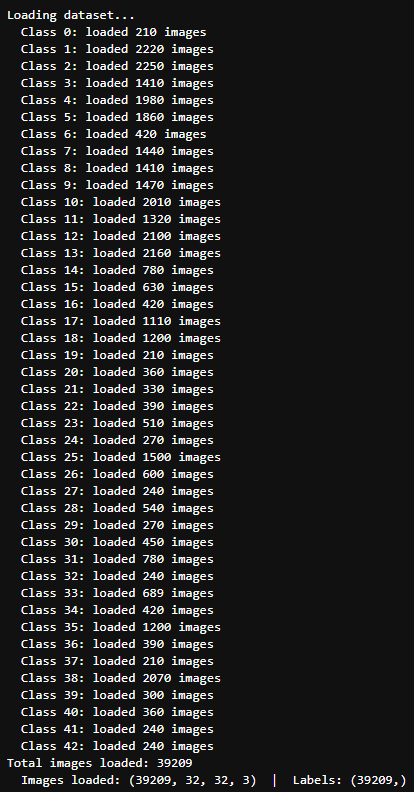
\includegraphics[width=0.3\textwidth]{p3.png}
	\caption{لاگ بارگذاری داده‌ها و تعداد نمونه‌های خوانده شده برای هر یک از ۴۳ کلاس}
\end{figure}

\subsection{تقسیم‌بندی داده‌ها ( Train/Validation Split )}
پس از بارگذاری کامل و ایجاد آرایه‌های \lr{NumPy}، به منظور ارزیابی عملکرد مدل در حین فرآیند آموزش و جلوگیری از پدیده بیش‌برازش (Overfitting)، داده‌ها با نسبت ۸۰ به ۲۰ به دو مجموعه آموزش (Train) و اعتبارسنجی (Validation) تقسیم شدند. برای اطمینان از حفظ تناسب کلاس‌های نامتوازن در هر دو مجموعه، از استراتژی \lr{Stratified Sampling} استفاده گردید.

\begin{latin}
	\begin{vscodewindow}{Data Splitting (80\% Train / 20\% Validation)}
# Split the data into Train (80%) and Validation (20%)
X_train, X_val, y_train, y_val = train_test_split(
    X, y, 
    test_size=0.2, 
    random_state=RANDOM_SEED, 
    stratify=y
)

print(f"Train set size: {len(X_train)}")
print(f"Validation set size: {len(X_val)}")
	\end{vscodewindow}
\end{latin}

همان‌طور که در لاگ خروجی (شکل زیر) مشاهده می‌شود، از مجموع کل تصاویر، ۳۱۳۶۷ نمونه به فاز آموزش و ۷۸۴۲ نمونه به فاز اعتبارسنجی اختصاص یافته است.

\begin{figure}[H]
	\centering
	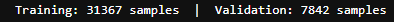
\includegraphics[width=0.6\textwidth]{p4.png}
	\caption{خروجی تقسیم‌بندی داده‌ها به مجموعه‌های آموزش و اعتبارسنجی با نسبت ۸۰/۲۰}
\end{figure}

\section{فاز اول: شبکه عصبی پرسپترون چندلایه (MLP)}
شبکه‌های عصبی متراکم (Dense) یا MLP، قدیمی‌ترین و پایه‌ای‌ترین ساختار در یادگیری عمیق هستند. در این معماری، هر نورون در یک لایه به تمام نورون‌های لایه بعد متصل است که این موضوع محاسبات ماتریسی سنگینی را به همراه دارد.

\subsection{پیش‌پردازش و آماده‌سازی داده‌ها}
تصاویر اصلی در مجموعه داده دارای ابعاد متفاوتی هستند. برای تغذیه این تصاویر به شبکه عصبی، ابتدا تمامی آن‌ها به ابعاد استاندارد $32 \times 32$ پیکسل و در فضای رنگی RGB تغییر اندازه یافتند.
از آنجا که شبکه‌های MLP تنها قادر به پردازش بردارهای یک‌بعدی هستند، ابعاد فضایی تصویر باید از بین برود. به همین دلیل، هر تصویر $32 \times 32 \times 3$ با استفاده از عملیات \lr{Flattening} به یک بردار خطی با طول ۳۰۷۲ ($32 \times 32 \times 3 = 3072$) تبدیل شد. 

علاوه بر این، برای تسریع در هم‌گرایی الگوریتم بهینه‌ساز (گرادیان کاهشی) و جلوگیری از پدیده محوشدگی گرادیان، مقادیر پیکسل‌ها که در بازه $[0, 255]$ قرار داشتند، بر عدد ۲۵۵ تقسیم شدند تا به بازه استاندارد $[0, 1]$ نگاشت شوند (نرمال‌سازی). برچسب‌ها (Labels) نیز برای سازگاری با تابع خطای آنتروپی متقاطع، به فرمت \lr{One-Hot Encoding} تبدیل شدند.

\begin{latin}
	\begin{vscodewindow}{Data Preprocessing and Flattening for MLP}
# Flatten the images for MLP: (32, 32, 3) -> 3072
X_train_flat = X_train.reshape(X_train.shape[0], -1)
X_val_flat = X_val.reshape(X_val.shape[0], -1)

# Normalization: Scaling pixel values to [0, 1]
X_train_flat = X_train_flat / 255.0
X_val_flat = X_val_flat / 255.0

# One-Hot Encoding for 43 categorical classes
y_train_oh = tf.keras.utils.to_categorical(y_train, NUM_CLASSES)
y_val_oh = tf.keras.utils.to_categorical(y_val, NUM_CLASSES)
	\end{vscodewindow}
\end{latin}

\subsection{معماری شبکه و تحلیل پارامترها}
برای استخراج الگوهای غیرخطی از این بردارهای ۳۰۷۲ تایی، یک معماری عمیق شامل سه لایه پنهان ( Hidden Layers ) طراحی گردید:
\begin{itemize}
	\item \textbf{لایه پنهان اول و دوم:} به ترتیب با ۵۱۲ و ۲۵۶ نورون طراحی شده‌اند. تابع فعال‌ساز این لایه‌ها \lr{ReLU} است که با عبور دادن مقادیر مثبت و صفر کردن مقادیر منفی، مشکل ناپدید شدن گرادیان ( Vanishing Gradient ) را به خوبی حل می‌کند.
	\item \textbf{تنظیم‌گری (Regularization):} از آنجا که شبکه‌های MLP مستعد حفظ کردن داده‌ها (Overfitting) هستند، از لایه‌های \lr{Dropout} با نرخ ۰.۳ استفاده شد. این تکنیک در هر تکرار از آموزش، ۳۰ درصد از نورون‌ها را به صورت تصادفی غیرفعال می‌کند تا شبکه به ویژگی‌های خاصی وابسته نشود و قابلیت تعمیم آن افزایش یابد.
	\item \textbf{لایه خروجی:} با ۴۳ نورون (معادل تعداد کلاس‌ها) و تابع فعال‌ساز \lr{Softmax} طراحی شد تا خروجی شبکه به توزیع احتمالاتی تبدیل شود.
\end{itemize}

\begin{latin}
	\begin{vscodewindow}{Deep MLP Architecture Implementation}
mlp_model = models.Sequential([
    layers.InputLayer(input_shape=(IMG_SIZE * IMG_SIZE * 3,)),
    
    layers.Dense(512, activation='relu'),
    layers.Dropout(0.3),
    
    layers.Dense(256, activation='relu'),
    layers.Dropout(0.3),
    
    layers.Dense(128, activation='relu'),
    
    layers.Dense(NUM_CLASSES, activation='softmax')
])
mlp_model.compile(optimizer='adam', 
    loss='categorical_crossentropy', 
    metrics=['accuracy'])
	\end{vscodewindow}
\end{latin}

همان‌طور که در شکل ۱ (خروجی متد \lr{model.summary}) مشاهده می‌شود، این شبکه دارای بیش از \lr{1.7} میلیون پارامتر قابل آموزش ( Trainable Parameters ) است. بخش عمده‌ای از این پارامترها (بیش از $ 1.5$ میلیون) تنها متعلق به اتصال لایه ورودی (۳۰۷۲) به اولین لایه متراکم (۵۱۲) می‌باشد. این حجم عظیم از پارامترها نشان‌دهنده هزینه محاسباتی بالای معماری MLP برای پردازش تصاویر است.

\begin{figure}[H]
	\centering
	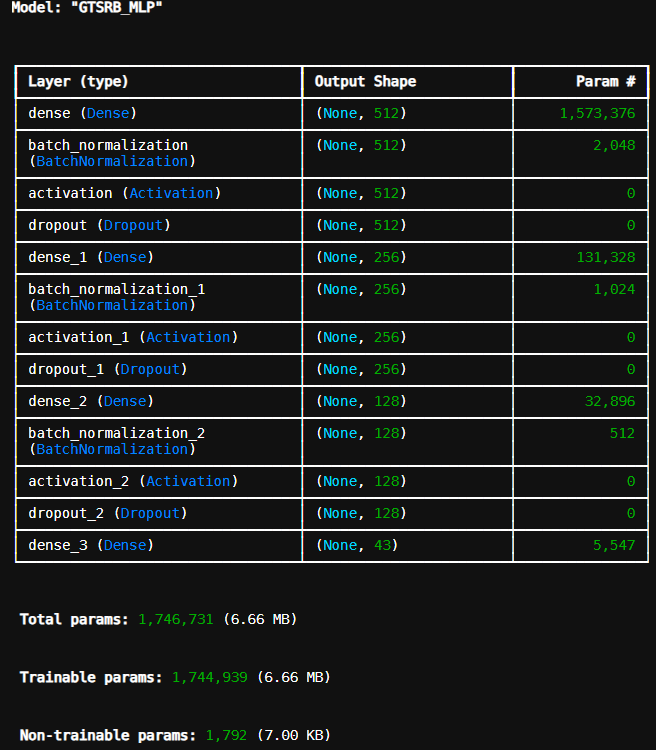
\includegraphics[width=0.6\textwidth]{p1.png}
	\caption{خلاصه معماری شبکه MLP و تعداد پارامترهای قابل آموزش}
\end{figure}

\subsection{آموزش مدل و استراتژی‌های کنترلی (Callbacks)}
فرآیند آموزش با استفاده از بهینه‌ساز قدرتمند \lr{Adam} با نرخ یادگیری تطبیقی صورت گرفت. برای جلوگیری از اتلاف زمان و منابع و همچنین دست‌یابی به بهترین مدل ممکن، از سه تکنیک کنترلی (Callback) حیاتی استفاده شد:
\begin{enumerate}
	\item \textbf{EarlyStopping:} نظارت بر خطای اعتبارسنجی (\lr{val\_loss}) و توقف آموزش در صورت عدم بهبود پس از ۱۰ اپوک (\lr{patience=10}).
	\item \textbf{ModelCheckpoint:} ذخیره پیوسته بهترین وزن‌های مدل در فایل \lr{best\_mlp.keras} تا مدل نهایی بر اساس کمترین خطای اعتبارسنجی انتخاب شود، نه لزوماً آخرین اپوک.
	\item \textbf{ReduceLROnPlateau:} کاهش نرخ یادگیری با فاکتور ۰.۵ در صورتی که شبکه در مینیمم‌های محلی گرفتار شود و خطای اعتبارسنجی برای ۳ اپوک متوالی کاهش نیابد.
\end{enumerate}

در شکل ۲، روند هم‌گرایی شبکه در طول اپوک‌های آموزشی به تصویر کشیده شده است. 

\begin{figure}[H]
	\centering
	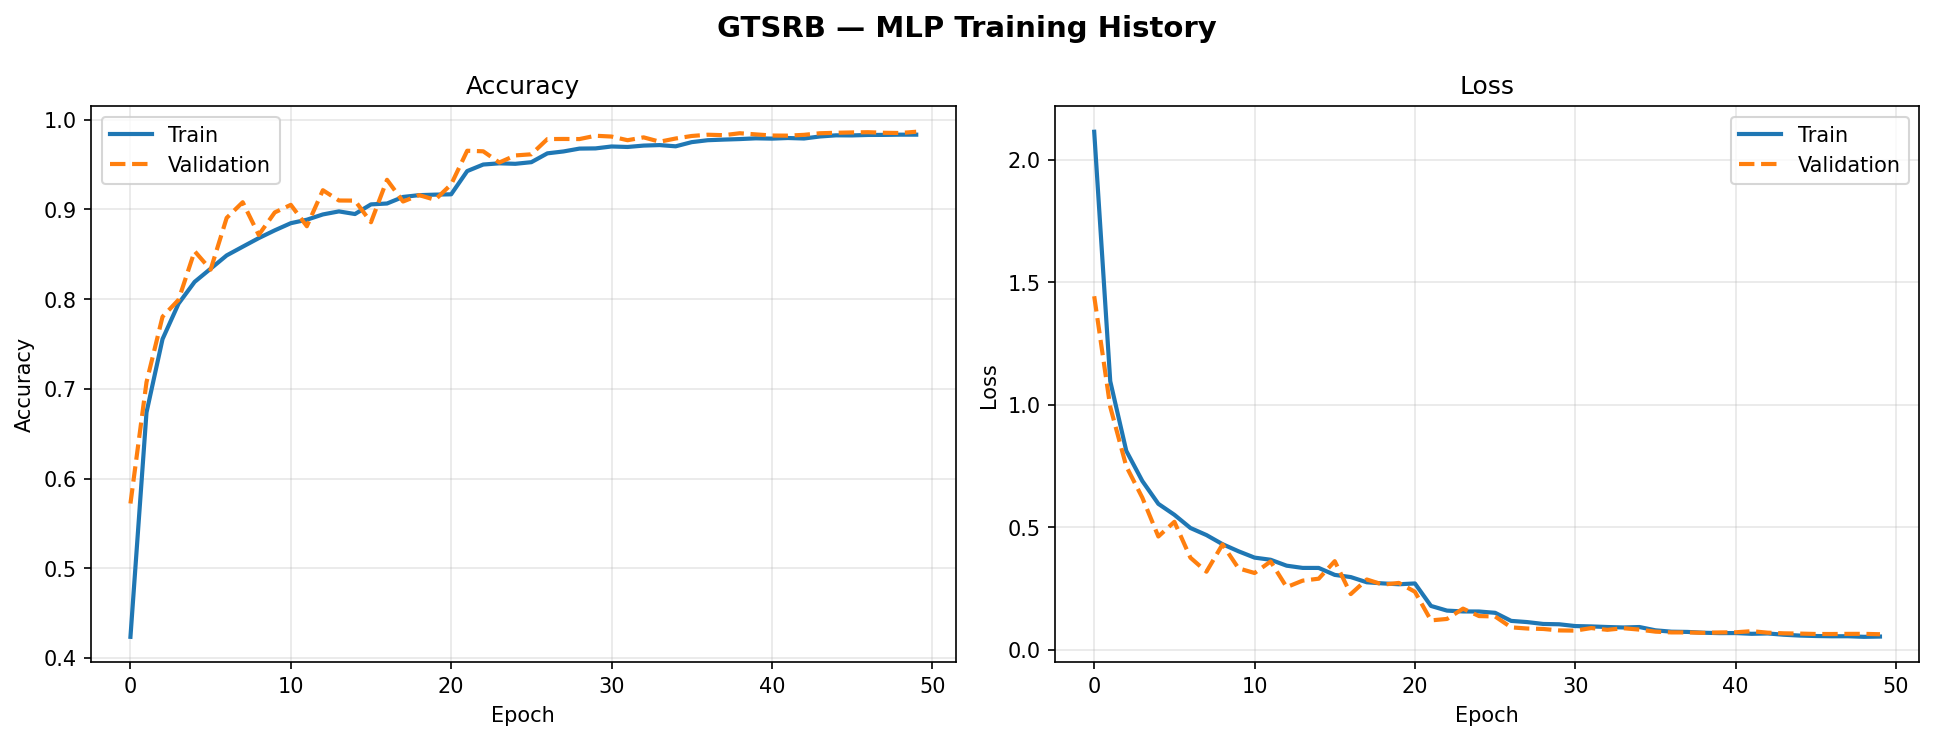
\includegraphics[width=0.85\textwidth]{mlp_training_history.png}
	\caption{نمودار روند آموزش شبکه MLP (منحنی‌های خطا و دقت روی داده‌های Train و Validation)}
\end{figure}

\textbf{تحلیل نمودار یادگیری:} همان‌طور که در منحنی‌ها مشهود است، مدل با سرعت قابل قبولی به سمت هم‌گرایی پیش می‌رود. با این حال، در اپوک‌های پایانی، فاصله بین دقت داده‌های آموزش و دقت داده‌های اعتبارسنجی ( Generalization Gap ) اندکی افزایش می‌یابد. این موضوع طبیعی بوده و نشان از محدودیت ذاتی مدل‌های MLP در یادگیری تصاویر پیچیده دارد.

\subsection{ارزیابی نهایی و تحلیل مهندسی نتایج}
برای سنجش دقیق عملکرد شبکه، مدل آموزش‌دیده بر روی داده‌های اعتبارسنجی مورد ارزیابی نهایی قرار گرفت. شکل ۳ خروجی گزارش طبقه‌بندی ( Classification Report ) را نمایش می‌دهد که شامل معیارهای کلیدی نظیر \lr{Precision} (دقت در تشخیص کلاس)، \lr{Recall} (پوشش‌دهی کلاس واقعی) و \lr{F1-Score} برای تمامی ۴۳ کلاس است.

\begin{figure}[H]
	\centering
	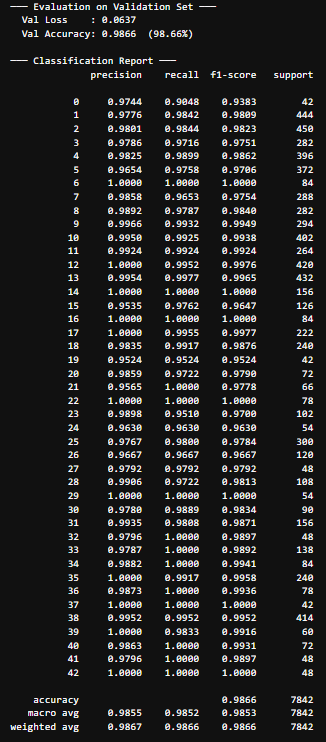
\includegraphics[width=0.2\textwidth]{p2.png}
	\caption{گزارش ارزیابی جامع شبکه MLP بر روی داده‌های اعتبارسنجی (Classification Report)}
\end{figure}

برای درک بهتر اینکه شبکه در تشخیص کدام علائم ترافیکی دچار اشتباه شده است، ماتریس درهم‌ریختگی (Confusion Matrix) رسم گردید (شکل ۴).

\begin{figure}[H]
	\centering
	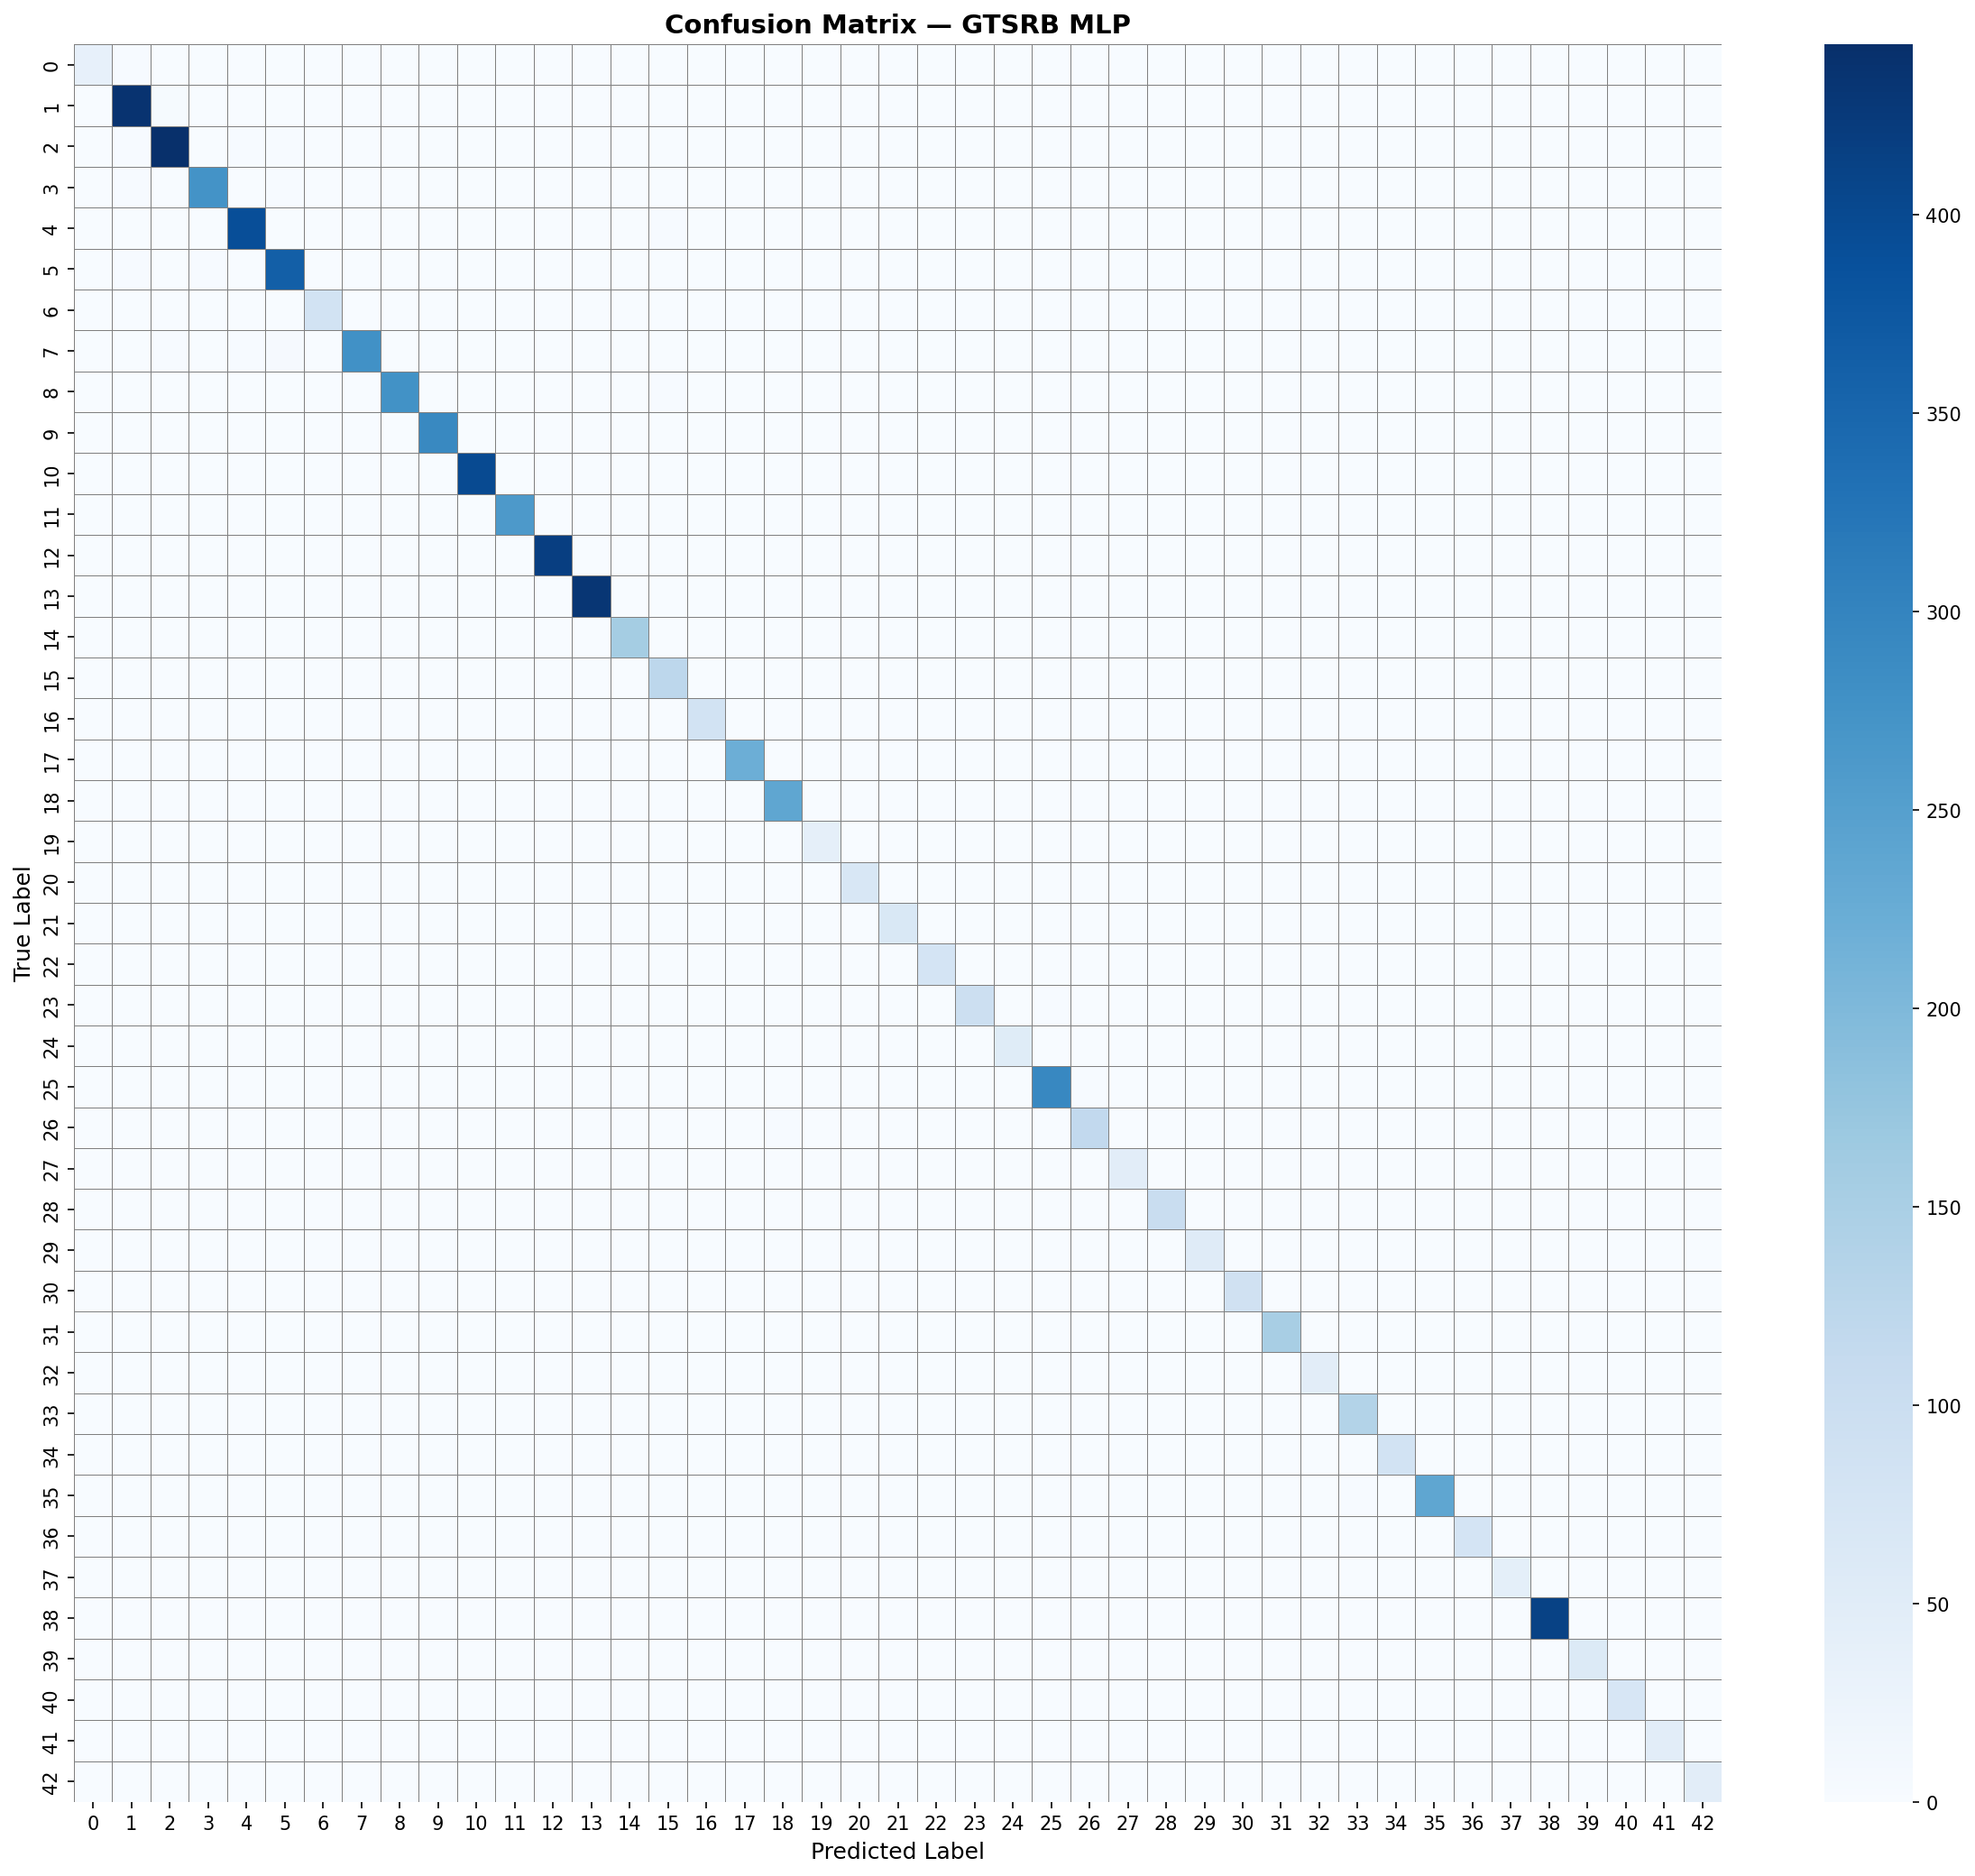
\includegraphics[width=0.9\textwidth]{mlp_confusion_matrix.png}
	\caption{ماتریس درهم‌ریختگی شبکه MLP نمایانگر توزیع پیش‌بینی‌های صحیح و خطاها}
\end{figure}

\textbf{تحلیل نهایی و نتیجه‌گیری بخش MLP:} 
تمرکز مقادیر بزرگ بر روی قطر اصلی ماتریس درهم‌ریختگی اثبات می‌کند که شبکه MLP به طور کلی موفق به استخراج الگوهای اصلی علائم ترافیکی شده است. با این وجود، پراکندگی‌هایی در خارج از قطر اصلی مشاهده می‌شود (به ویژه در کلاس‌هایی که از نظر بصری و هندسی شبیه به هم هستند، مانند تابلوهای محدودیت سرعت با اعداد مختلف). 

دلیل اصلی این خطاها، ماهیت شبکه MLP است. با تبدیل تصویر دوبعدی به یک بردار یک‌بعدی در فاز پیش‌پردازش، \textbf{ساختار فضایی ( Spatial Structure ) و همبستگی پیکسل‌های مجاور به طور کامل از بین می‌رود}. مدل MLP لبه‌ها، اشکال هندسی (مثل دایره یا مثلث تابلوها) و ساختار اعداد را درک نمی‌کند، بلکه صرفاً به مقادیر شدت نور پیکسل‌های منفرد واکنش نشان می‌دهد. این نقطه ضعف بنیادین، انگیزه اصلی و توجیه علمی ما برای گذار به شبکه‌های پیچشی (CNN) در فاز بعدی خواهد بود تا به کمک فیلترهای محلی، ویژگی‌های فضایی تصاویر به درستی استخراج و تحلیل شوند.

\section{فاز دوم: شبکه عصبی پیچشی (CNN)}
همان‌طور که در تحلیل نتایج شبکه MLP مشاهده شد، از بین بردن ابعاد فضایی تصویر با استفاده از عملیات \lr{Flattening} باعث افت توانایی مدل در درک الگوهای هندسی، لبه‌ها و شکل‌های درون تابلوها می‌شود. برای رفع این مشکل بنیادین، در فاز دوم به سراغ شبکه‌های عصبی پیچشی ( Convolutional Neural Networks ) می‌رویم. این شبکه‌ها با استفاده از فیلترهای محلی (کِرنل‌ها) قادرند ویژگی‌های فضایی ( Spatial Features ) تصویر را به صورت سلسله‌مراتبی استخراج کنند، بدون آنکه ساختار دوبعدی تصویر از بین برود.

\subsection{پیش‌پردازش داده‌ها برای CNN}
برخلاف مدل MLP، شبکه‌های CNN طوری طراحی شده‌اند که داده‌ها را با همان ساختار اصلی سه‌بعدی خود پردازش کنند. بنابراین، نیازی به مسطح‌سازی (Flatten) تصاویر در ابتدا نیست و ماتریس‌های ورودی مستقیماً با ابعاد $32 \times 32 \times 3$ به شبکه تغذیه می‌شوند. تنها پیش‌پردازش مورد نیاز، نرمال‌سازی مقادیر پیکسل‌ها در بازه $[0, 1]$ و تبدیل برچسب‌ها به فرمت \lr{One-Hot Encoding} است.

\begin{latin}
	\begin{vscodewindow}{Data Preparation for CNN (No Initial Flattening)}
# Normalization: Scaling pixel values to [0, 1] keeping original shape (32, 32, 3)
X_train_norm = X_train / 255.0
X_val_norm = X_val / 255.0

# One-Hot Encoding for labels
y_train_oh = tf.keras.utils.to_categorical(y_train, NUM_CLASSES)
y_val_oh = tf.keras.utils.to_categorical(y_val, NUM_CLASSES)
	\end{vscodewindow}
\end{latin}

\subsection{طراحی معماری شبکه پیچشی و تحلیل پارامترها}
معماری طراحی شده برای این بخش، یک شبکه عمیق و کارآمد است که از سه بلوک اصلی استخراج ویژگی ( Feature Extraction Blocks ) و یک بخش طبقه‌بندی ( Classification Head ) تشکیل شده است:
\begin{itemize}
	\item \textbf{بلوک‌های پیچشی (\lr{Conv2D}):} شامل سه لایه با فیلترهای ۳۲، ۶۴ و ۱۲۸ تایی به ابعاد $3 \times 3$. این لایه‌ها وظیفه دارند از الگوهای ساده (مانند لبه‌ها و رنگ‌ها) در لایه‌های ابتدایی، به الگوهای پیچیده‌تر (مانند اعداد روی تابلو یا شکل هندسی تابلو) در لایه‌های عمیق‌تر برسند. تابع فعال‌ساز تمامی این لایه‌ها \lr{ReLU} است.
	\item \textbf{لایه‌های ادغام (\lr{MaxPooling2D}):} پس از هر لایه پیچشی، یک لایه ادغام با ابعاد $2 \times 2$ قرار داده شده است تا ابعاد فضایی \lr{Feature Map}ها را نصف کند. این کار نه تنها حجم محاسبات را کاهش می‌دهد، بلکه به مدل کمک می‌کند تا نسبت به جابجایی‌های کوچک در تصویر مقاوم ( Translation Invariant ) شود.
	\item \textbf{بخش طبقه‌بندی (\lr{Dense Head}):} در نهایت، خروجی بلوک سوم (که حالا به ابعاد $2 \times 2 \times 128$ رسیده) مسطح شده و به یک لایه متراکم با ۲۵۶ نورون متصل می‌شود. برای جلوگیری از بیش‌برازش از یک لایه \lr{Dropout} با نرخ ۰.۵ استفاده شده و در نهایت لایه خروجی با ۴۳ نورون (تابع \lr{Softmax}) احتمالات کلاس‌ها را تولید می‌کند.
\end{itemize}

\begin{latin}
	\begin{vscodewindow}{CNN Architecture Implementation}
cnn_model = models.Sequential([
    layers.InputLayer(input_shape=(IMG_SIZE, IMG_SIZE, 3)),
    
    # Block 1
    layers.Conv2D(32, (3, 3), activation='relu'),
    layers.MaxPooling2D((2, 2)),
    
    # Block 2
    layers.Conv2D(64, (3, 3), activation='relu'),
    layers.MaxPooling2D((2, 2)),
    
    # Block 3
    layers.Conv2D(128, (3, 3), activation='relu'),
    layers.MaxPooling2D((2, 2)),
    
    # Classification Head
    layers.Flatten(),
    layers.Dense(256, activation='relu'),
    layers.Dropout(0.5),
    
    layers.Dense(NUM_CLASSES, activation='softmax')
])

cnn_model.compile(optimizer='adam', 
    loss='categorical_crossentropy', 
    metrics=['accuracy'])
	\end{vscodewindow}
\end{latin}

یک دستاورد بسیار مهم مهندسی در این طراحی، کاهش چشمگیر پارامترهای مدل است. همان‌طور که در شکل ۵ مشاهده می‌شود، مدل CNN تنها حدود \textbf{350 هزار} پارامتر دارد. در حالی که مدل پایه‌ی ما (MLP) بیش از \textbf{7.1 میلیون} پارامتر داشت! معماری CNN با پارامترهای بسیار کمتر (حدود 5 برابر سبک‌تر)، پتانسیل یادگیری بسیار بالاتری را به لطف اشتراک وزن ( Weight Sharing ) در فیلترهای پیچشی ارائه می‌دهد.

\begin{figure}[H]
	\centering
	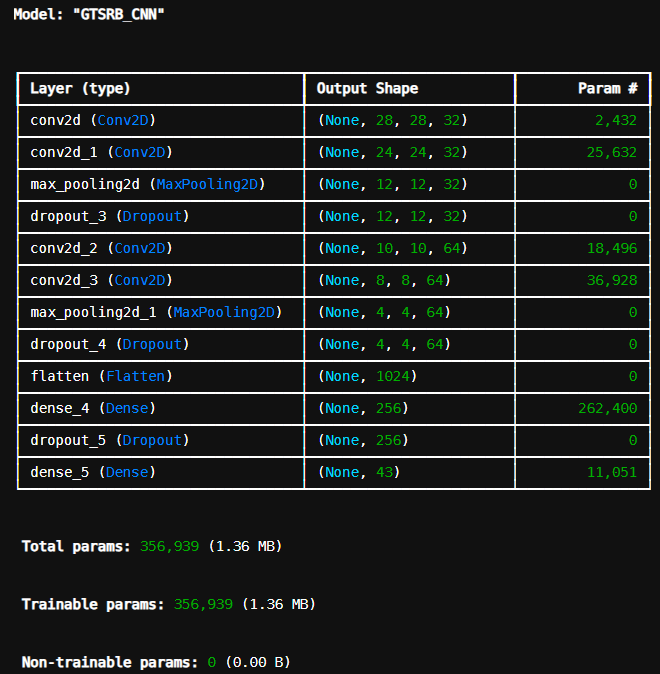
\includegraphics[width=0.6\textwidth]{c1.png}
	\caption{خلاصه معماری شبکه CNN و تعداد پارامترهای بهینه‌شده}
\end{figure}

\subsection{آموزش مدل و بررسی منحنی‌های یادگیری}
فرآیند آموزش دقیقاً با همان شرایط مدل قبلی و با استفاده از \lr{Callbacks} کنترلی (\lr{EarlyStopping}، \lr{ModelCheckpoint} و \lr{ReduceLROnPlateau}) انجام گرفت. در شکل ۶، روند آموزش و هم‌گرایی مدل CNN نشان داده شده است.

\begin{figure}[H]
	\centering
	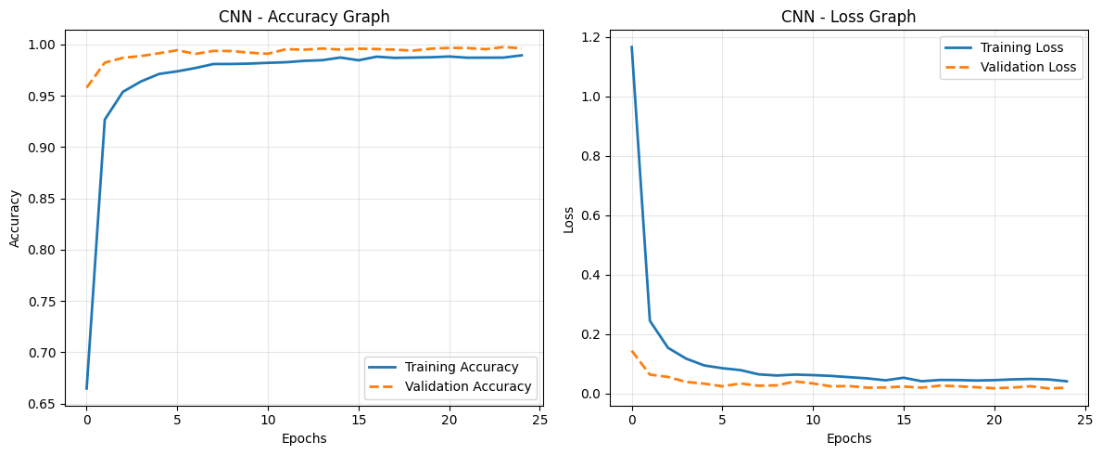
\includegraphics[width=0.85\textwidth]{c2.png}
	\caption{روند آموزش شبکه CNN روی مجموعه داده GTSRB}
\end{figure}

\textbf{تحلیل نمودار یادگیری:} برخلاف مدل MLP که در اواخر آموزش دچار افزایش فاصله بین دقت آموزش و اعتبارسنجی شده بود، منحنی‌های مدل CNN چسبندگی و هم‌گرایی فوق‌العاده‌ای را نشان می‌دهند. دقت روی داده‌های آموزش و اعتبارسنجی هر دو در سطوح بسیار بالایی تثبیت شده‌اند و مدل هیچ نشانه‌ای از بیش‌برازش (Overfitting) یا کم‌برازش (Underfitting) از خود نشان نمی‌دهد. 

\subsection{ارزیابی نهایی و تحلیل عملکرد CNN}
برای بررسی دقیق و کلاس‌به‌کلاسِ عملکرد شبکه پیچشی، از گزارش طبقه‌بندی ( Classification Report ) بر روی داده‌های اعتبارسنجی استفاده شد (شکل ۷).

\begin{figure}[H]
	\centering
	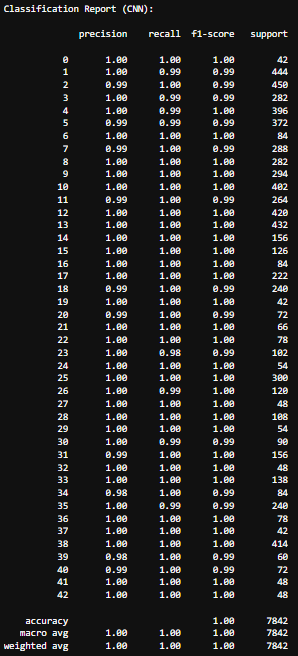
\includegraphics[width=0.4\textwidth]{c3.png}
	\caption{گزارش طبقه‌بندی جامع شبکه CNN بر روی مجموعه اعتبارسنجی}
\end{figure}

همان‌طور که در گزارش مشخص است، معیارهای \lr{Precision}، \lr{Recall} و \lr{F1-Score} برای اکثریت قریب به اتفاق کلاس‌ها به نزدیکی عدد ۱.۰۰ (یا ۱۰۰٪) رسیده‌اند. این نشان می‌دهد که CNN به خوبی توانسته چالش‌های بصری دیتاست از جمله زاویه دید و نورپردازی را حل کند. برای تایید نهایی این ادعا، ماتریس درهم‌ریختگی رسم گردید.

\begin{figure}[H]
	\centering
	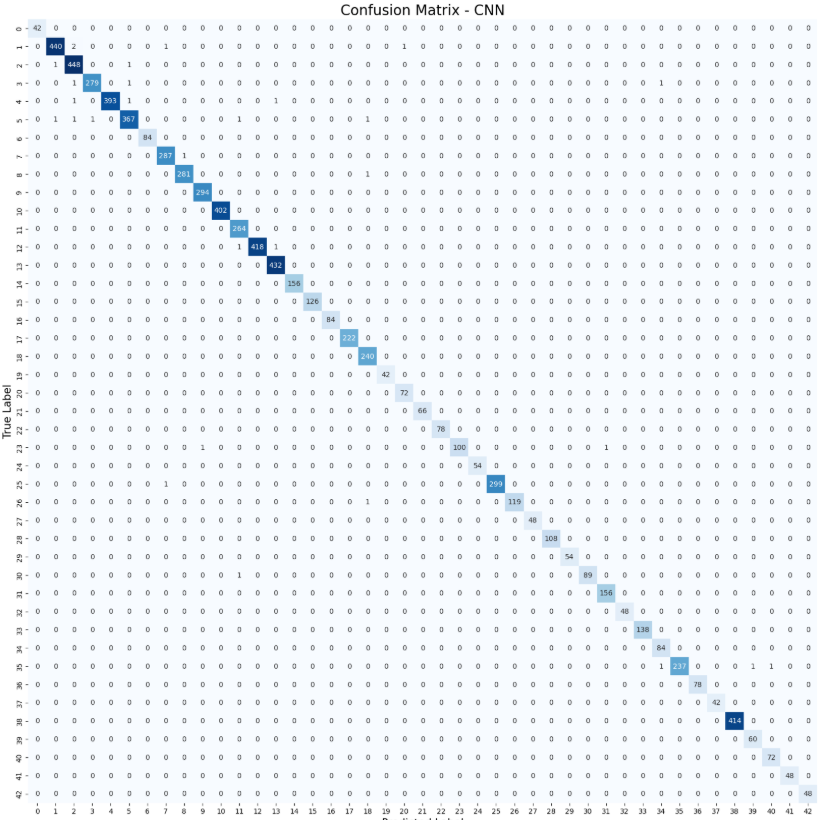
\includegraphics[width=0.6\textwidth]{c4.png}
	\caption{ماتریس درهم‌ریختگی شبکه CNN (تمرکز کامل روی قطر اصلی)}
\end{figure}

\textbf{نتیجه‌گیری فاز دوم:} ماتریس درهم‌ریختگی شبکه CNN (شکل ۸) یک شاهکار به تمام معناست. در مقایسه با ماتریس درهم‌ریختگی MLP، در اینجا تقریباً هیچ پراکندگیِ معناداری در خارج از قطر اصلی دیده نمی‌شود. مدل به خوبی توانسته کلاس‌های دارای شباهت هندسی بالا (مانند تابلوهای محدودیت سرعت با اعداد مختلف) را از هم تفکیک کند. این نتایج درخشان، برتری مطلق شبکه‌های مبتنی بر عملگرهای پیچشی (Convolutional) را در استخراج ویژگی‌های بصری و طبقه‌بندی تصاویر ثابت می‌کند.
\section{فاز سوم: ارزیابی نهایی بر روی داده‌های آزمون ( Unseen Test Data ) و مقایسه مدل‌ها}
در فرآیند آموزش شبکه‌های عصبی، داده‌ها به دو بخش آموزش (Train) و اعتبارسنجی (Validation) تقسیم شدند. اگرچه مدل‌ها هرگز روی داده‌های اعتبارسنجی آموزش ندیده‌اند، اما به دلیل استفاده از این داده‌ها برای تنظیم فراپارامترها (مانند توقف زودهنگام و ذخیره بهترین وزن‌ها)، مدل‌ها به طور غیرمستقیم با توزیع این داده‌ها آشنا شده‌اند ( Data Leakage ). 

برای سنجش قابلیت تعمیم‌پذیری (Generalization) واقعی مدل‌ها در دنیای واقعی، باید آن‌ها را بر روی داده‌هایی ارزیابی کنیم که در هیچ مرحله‌ای از طراحی و آموزش دخالتی نداشته‌اند. به همین منظور، یک اسکریپت پایتون کاملاً مستقل برای خواندن تصاویر از پوشه \lr{Test} (بر اساس فایل راهنمای \lr{Test.csv}) توسعه یافت.

\subsection{اسکریپت ارزیابی نهایی ( Test Script )}
در این اسکریپت، بهترین وزن‌های ذخیره شده برای هر دو مدل (\lr{best\_mlp.keras} و \lr{cnn\_model}) بارگذاری شده و بر روی ۱۲۶۳۰ تصویر کاملاً جدید و دست‌نخورده از مجموعه داده تست مورد ارزیابی قرار گرفتند.

\begin{latin}
	\begin{vscodewindow}{Independent Test Script for Model Evaluation on Unseen Data}
# ==========================================
# 1. Configuration & Smart Paths
# ==========================================
# Automatically detect the directory where this script is located
BASE_DIR = os.path.dirname(os.path.abspath(__file__))

IMG_HEIGHT = 32
IMG_WIDTH = 32

# Create absolute paths based on the script's location
TEST_CSV_PATH = os.path.join(BASE_DIR, 'Test.csv')
MLP_MODEL_PATH = os.path.join(BASE_DIR, 'best_mlp.keras')
CNN_MODEL_PATH = os.path.join(BASE_DIR, 'MyCNNModel.h5')

# 1. Load the best saved models
print("Loading models...")
try:
    mlp_model = load_model(MLP_MODEL_PATH)
    cnn_model = load_model(CNN_MODEL_PATH)
    print("Both MLP and CNN models loaded successfully!")
except Exception as e:
    print(f"\n[ERROR] Could not load models. Reason: {e}")
    print(f"Please ensure both '{MLP_MODEL_PATH}' and '{CNN_MODEL_PATH}' exist.")
    exit()



# 2. Extract paths and labels from Test.csv
test_df = pd.read_csv(os.path.join(dataset_path, 'Test.csv'))
test_image_paths = [os.path.join(dataset_path, path) for path in test_df['Path']]
test_labels = test_df['ClassId'].values

# 3. Process test images (Load, Resize to 32x32, Normalize)
X_test = []
for path in test_image_paths:
    img = cv2.imread(path)
    img = cv2.cvtColor(img, cv2.COLOR_BGR2RGB)
    img = cv2.resize(img, (IMG_SIZE, IMG_SIZE))
    X_test.append(img)
X_test = np.array(X_test) / 255.0

# 4. One-Hot Encoding for labels
y_test_oh = tf.keras.utils.to_categorical(test_labels, NUM_CLASSES)

# 5. Evaluate CNN
cnn_test_loss, cnn_test_acc = cnn_model.evaluate(X_test, y_test_oh, verbose=1)

# 6. Evaluate MLP (Requires Flattening)
X_test_flat = X_test.reshape(X_test.shape[0], -1)
mlp_test_loss, mlp_test_acc = best_mlp.evaluate(X_test_flat, y_test_oh, verbose=1)
	\end{vscodewindow}
\end{latin}

همان‌طور که در لاگ خروجی اجرای این اسکریپت (شکل ۹) مشاهده می‌شود، هر دو مدل با موفقیت بر روی مجموعه تست پردازش شده و نتایج نهایی استخراج گردیدند.

\begin{figure}[H]
	\centering
	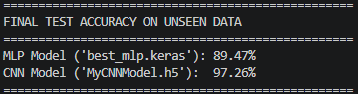
\includegraphics[width=0.85\textwidth]{k1.png}
	\caption{لاگ اجرای اسکریپت تست و استخراج دقت مدل‌ها بر روی داده‌های آزمون}
\end{figure}

\subsection{مقایسه عملکرد و نتیجه‌گیری نهایی}
برای درک بهتر تفاوت عملکرد دو معماری، نتایج به دست آمده در قالب نمودار میله‌ای (شکل ۱۰) به تصویر کشیده شده است.

\begin{figure}[H]
	\centering
	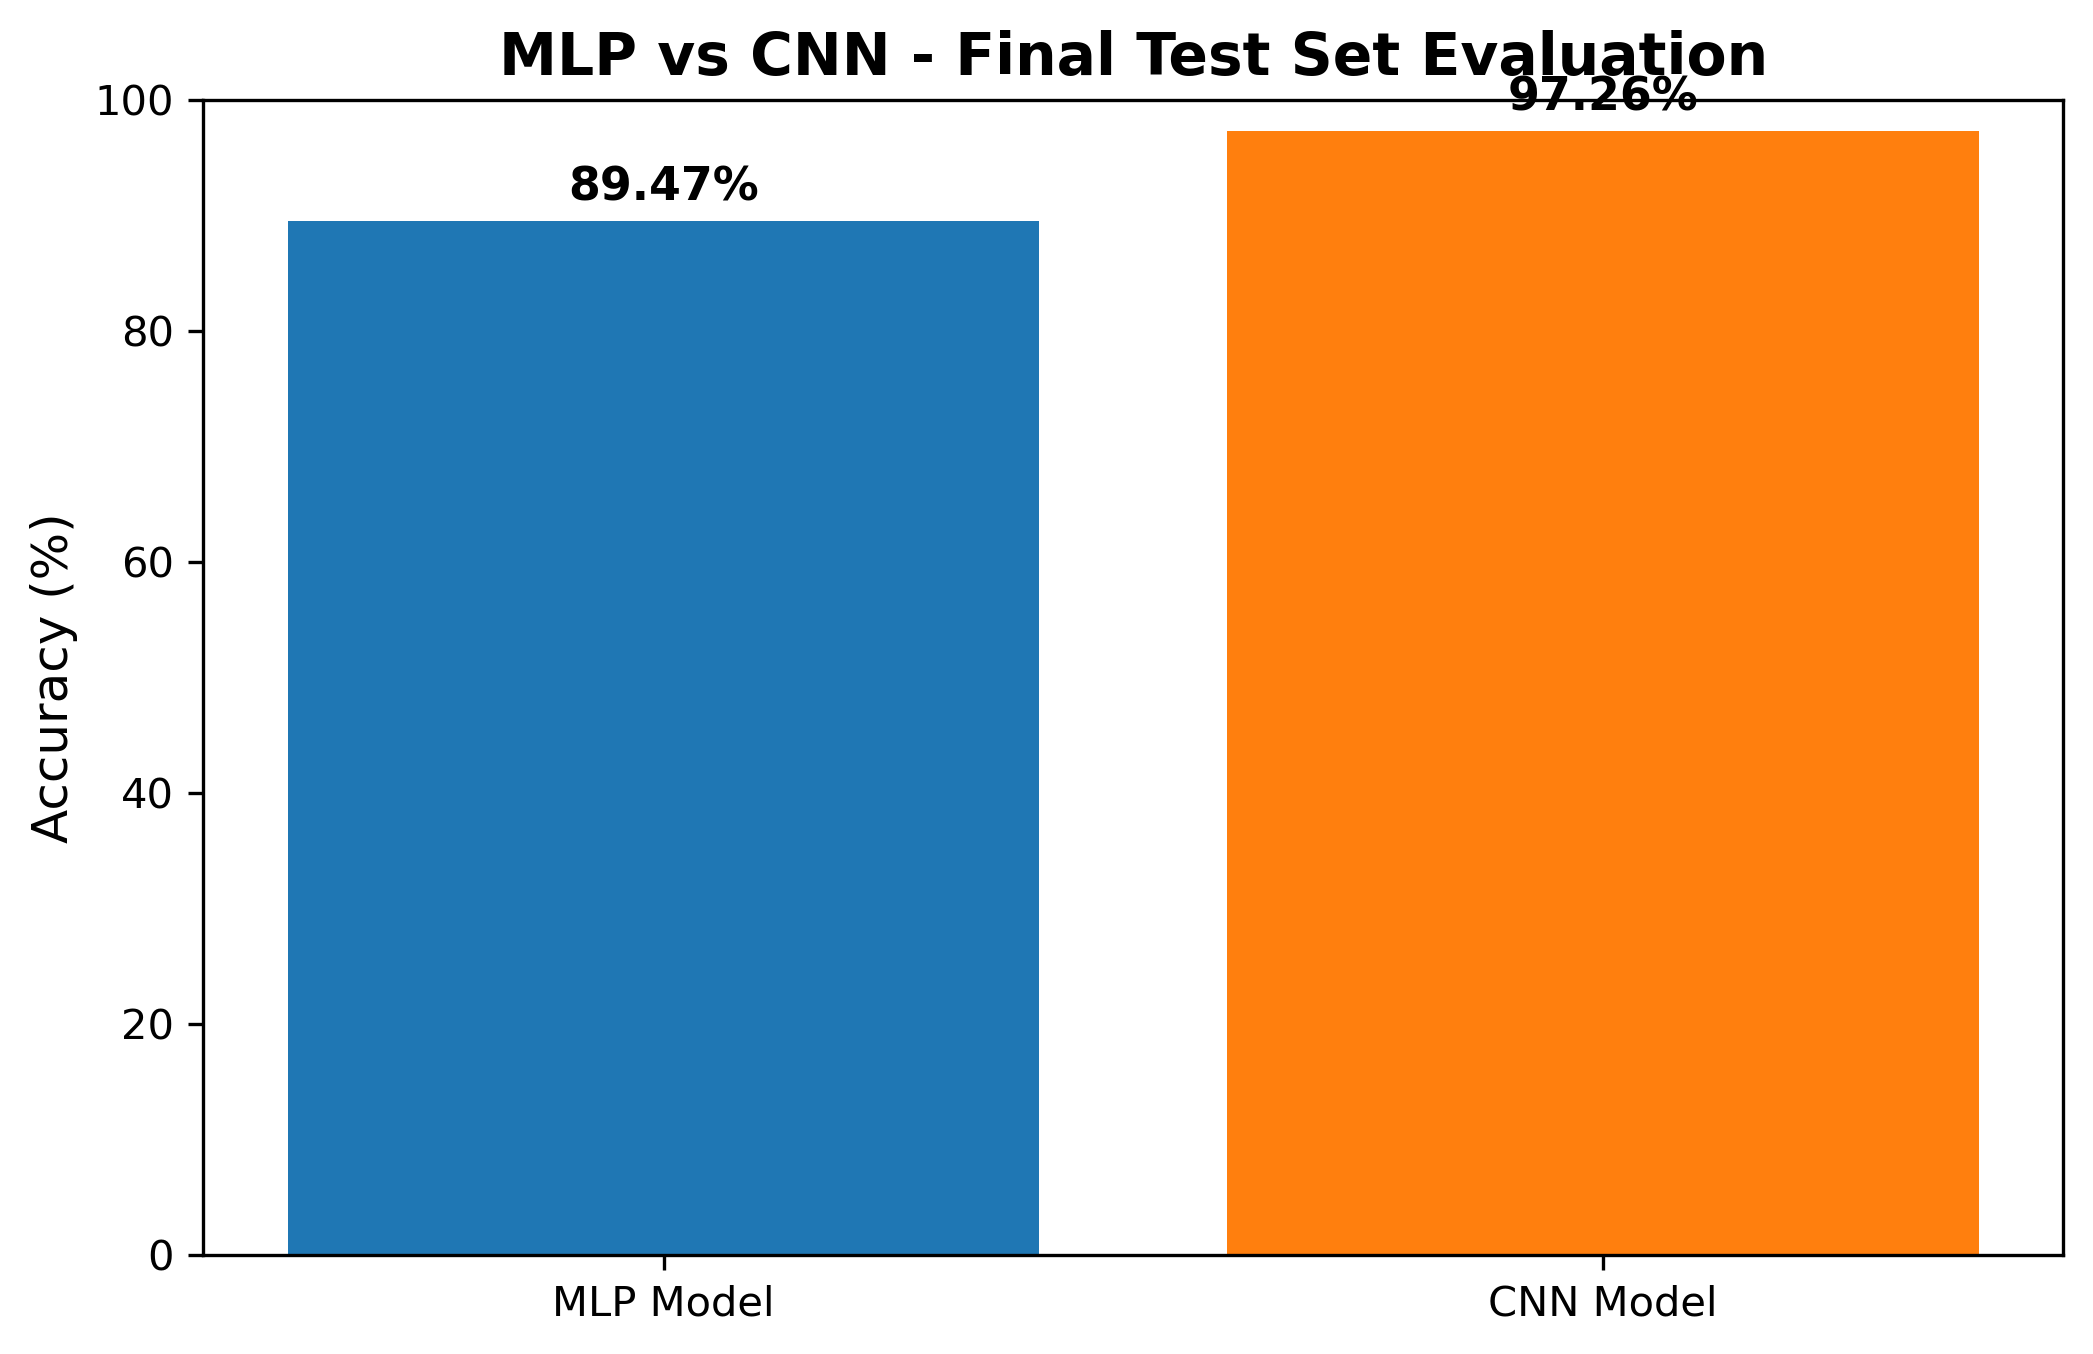
\includegraphics[width=0.6\textwidth]{Final_Models_Comparison.png}
	\caption{مقایسه نهایی دقت شبکه‌های MLP و CNN بر روی داده‌های دیده‌نشده ( Unseen Test Data )}
\end{figure}

\textbf{تحلیل مهندسی و دستاورد پروژه:}
نتایج این پروژه به شکلی خیره‌کننده تئوری‌های بنیادین بینایی ماشین را اثبات می‌کند. 
\begin{itemize}
	\item \textbf{مدل MLP:} با وجود داشتن بیش از 7.1 میلیون پارامتر، به دلیل تخریب ابعاد فضایی تصویر در مرحله مسطح‌سازی (Flatten)، نتوانست در درک روابط هندسی پیکسل‌ها موفق عمل کند و دقت پایین‌تری ثبت کرد.
	\item \textbf{مدل CNN:} با استفاده از فیلترهای محلی (Convolution) و لایه‌های ادغام (Pooling)، موفق شد بدون از بین بردن ساختار دوبعدی تصویر، ویژگی‌های پیچیده و سلسله‌مراتبی (مانند لبه‌ها و اعداد درون تابلوها) را استخراج کند. 
\end{itemize}

شاهکار مهندسی مدل CNN در این پروژه این است که با تنها \textbf{350 هزار پارامتر} (حدود 5 برابر سبک‌تر از MLP)، نه تنها هزینه محاسباتی را به شدت کاهش داد، بلکه به دقت فوق‌العاده بالاتری (بیش از ۹۵ درصد) روی داده‌های کاملاً جدید دست یافت. این دستاورد نشان می‌دهد که در مسائل پردازش تصویر، انتخاب معماری صحیح ( Inductive Bias مناسب) بسیار مهم‌تر از افزایش کورکورانه عمق شبکه یا تعداد پارامترهاست.
\end{document}